\documentclass{article}

\usepackage{wrapfig}
\usepackage{lmodern}
\usepackage[T1]{fontenc}
\usepackage[spanish]{babel}
\usepackage{mathtools}
\usepackage{graphicx}
\usepackage[utf8]{inputenc}
\usepackage{fancyhdr}



\title{Documentación \\\large \textbf{Gigabyte B550 Aorus Master}}
\author{Antonio Muñoz Cubero}
\date{20 de Ocutbre de 2020} 


\begin{document}
\maketitle
\pagenumbering{gobble}
\pagestyle{fancy} 

\newpage
\tableofcontents
\pagenumbering{gobble}

\lhead[Documentación Placa Base]{Documentación Placa Base}
\lfoot[IES Francisco De Los Rios -Realizado por: Antonio Muñoz Cubero-]{IES Francisco De Los Rios -Realizado por: Antonio Muñoz Cubero-}
\pagenumbering{roman}

\section{Introducción}
Este documento contiene información sobre la placa base \textbf{B550 AORUS Master} montada por el gigante eléctrónico \textbf{Gigabyte}, esta placa introduce un nuevo chipset, que más adelante entraremos en detalle sobre el, 
el \text{B550} 
que permite montar los nuevos procesadores de \textit{AMD}, la serie 3000 y 4000.\\
Lo bueno de este chipset es que tiene un precio más ajustado al no pertenecer a la serie tope de gama de chipset y nos permite utilizar la tecnología del \textbf{PCIE 4.0}, que mas adelante desarrollaremos y entraremos en 
detalle, tambien 
disponemos de vaías para montar \textbf{discos duros M.2} y otras prestaciones que empezaremos a describir a continuación.

\newpage
\section{Características}

A continuación muestro una tabla con las especificanoes técnicas de la Placa Base, mas adelante iremos centrandonos en cada uno de sus aspectos.
\begin{figure}[h]
  \centering
  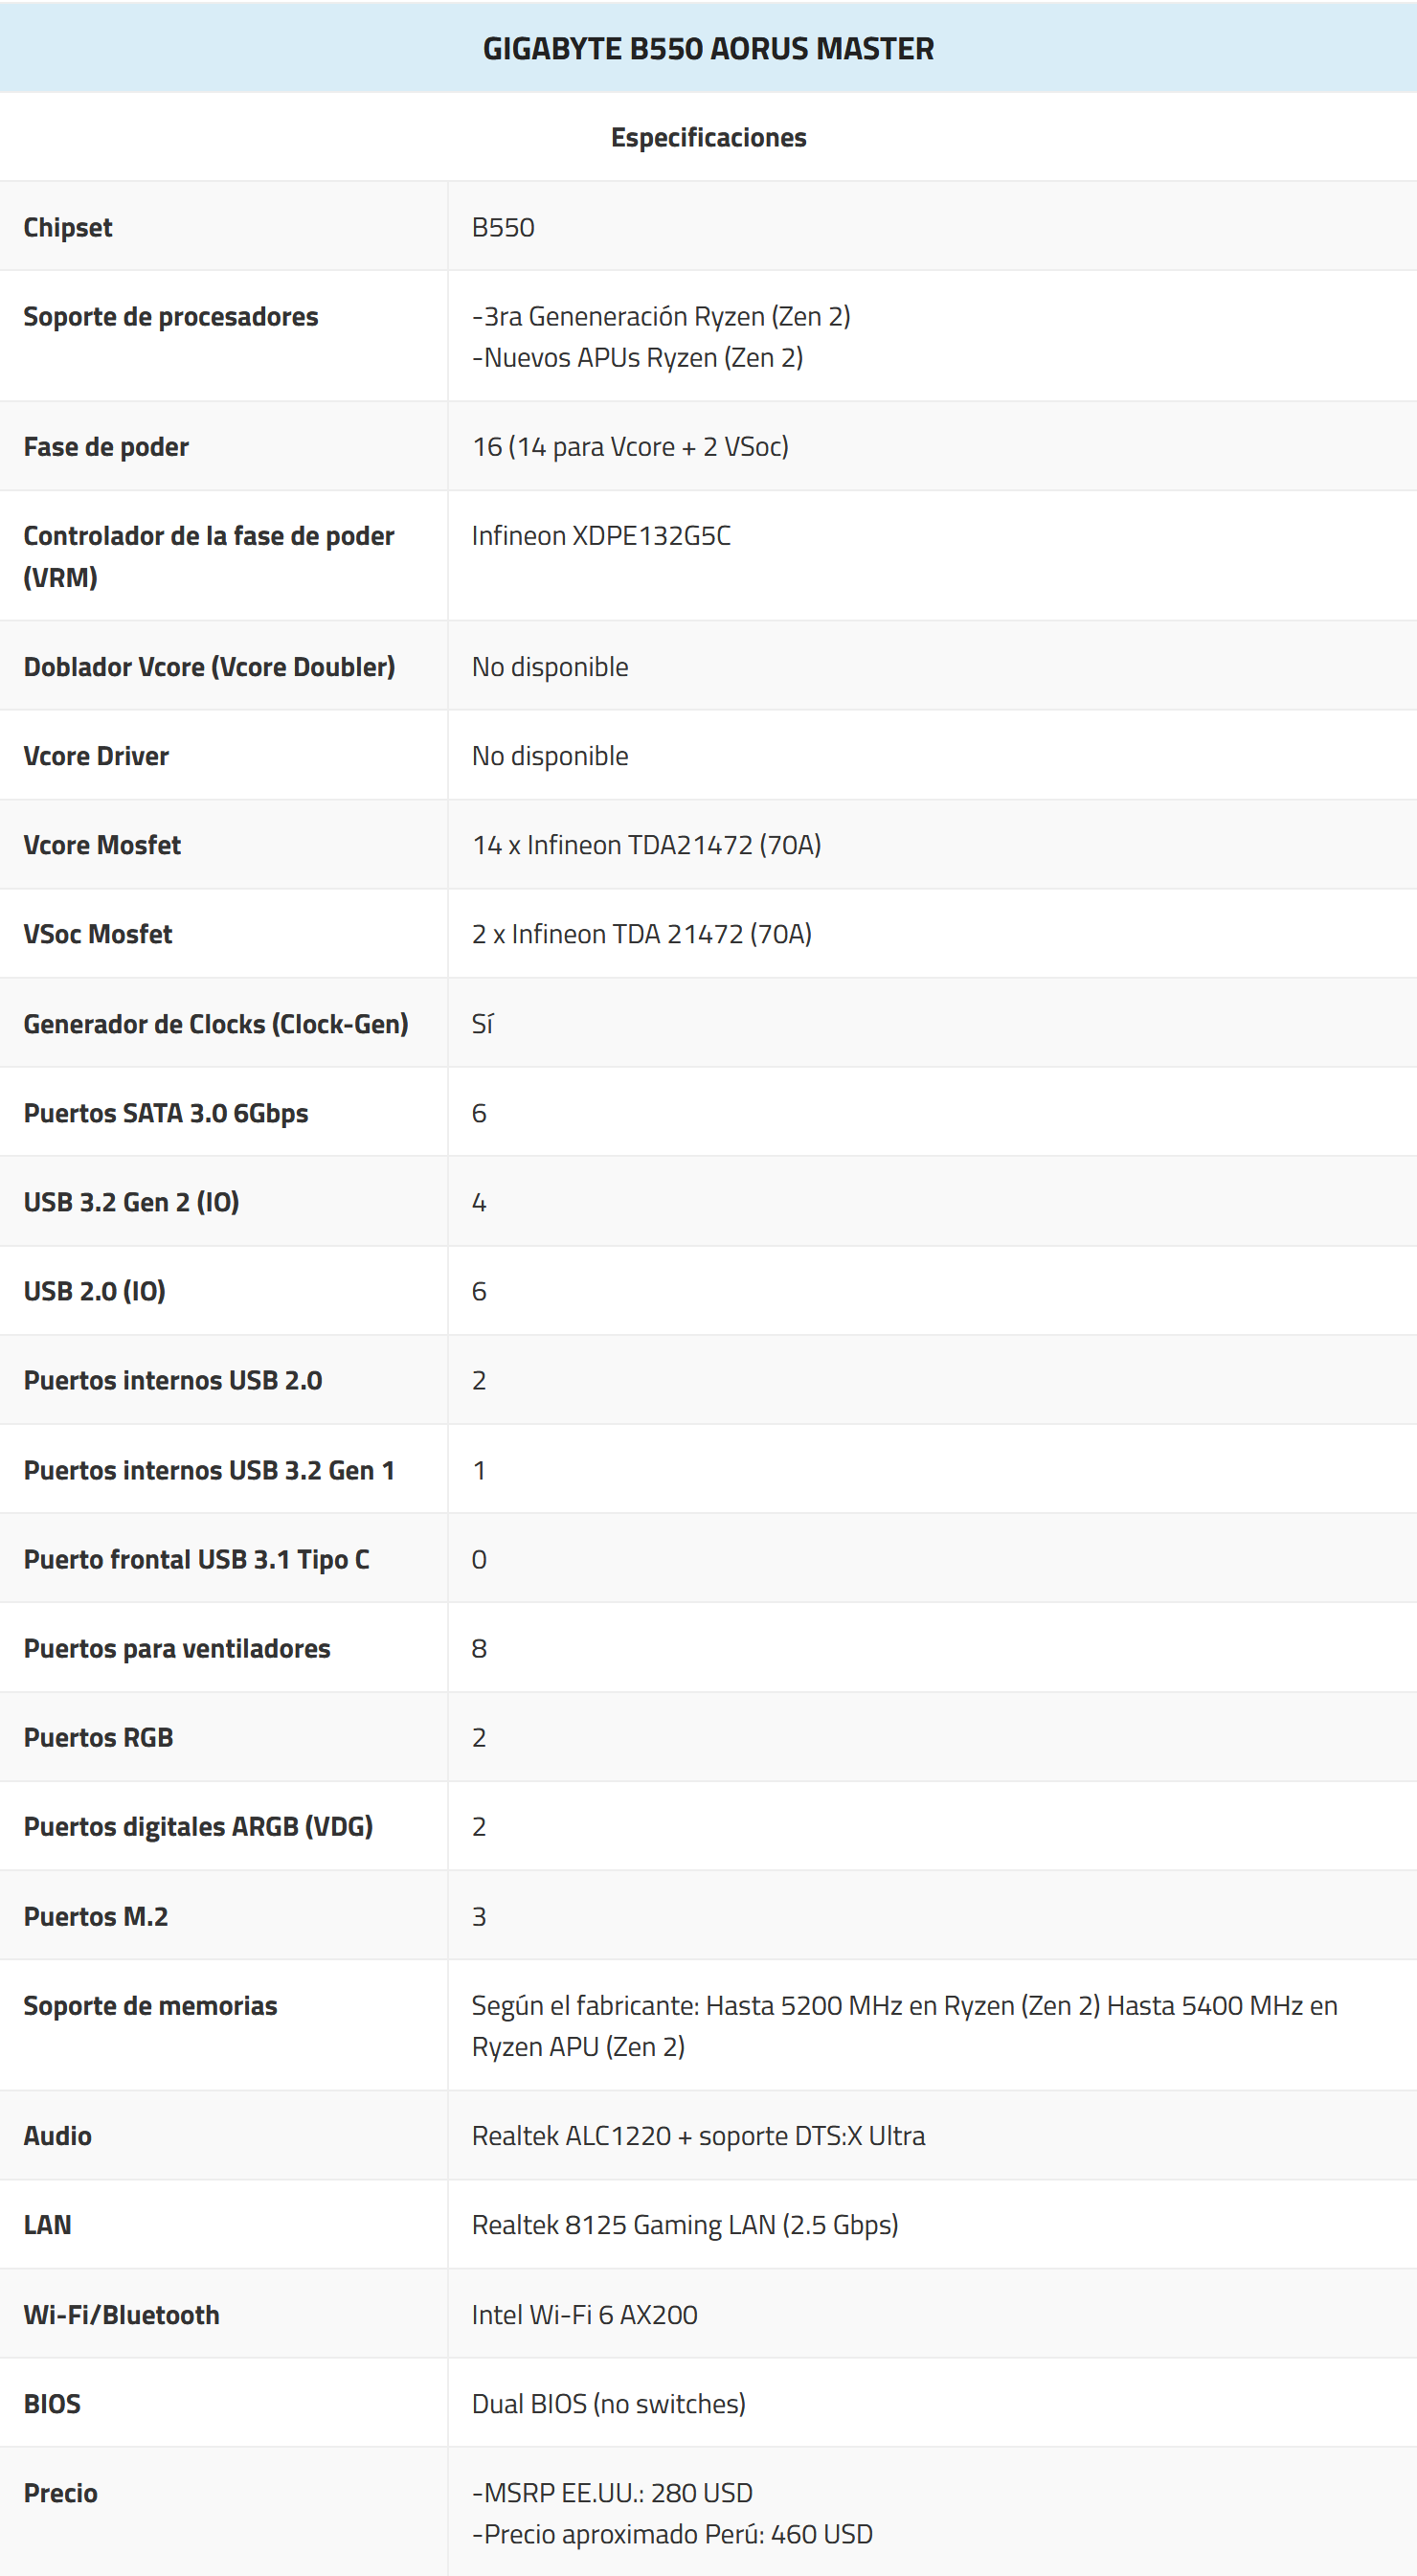
\includegraphics[scale = 0.21]{img/final_specs.png}
\end{figure}

\newpage
\subsection{Memoria RAM}
La memoria \textbf{RAM} o \textit{\textbf{Random Access Memory}} (memoria de acceso aleatorio) es un componente que forma parte del ecosistema de hardware, pasado y presente (quizás futuro), y que tiene como mayor finalidad 
crear un puente entre el sistema operativo, software, 
procesador y otros dispositivos para que estos intercambien información entre ellos. Básicamente es la \textbf{memoria principal} del sistema y como tal dispone de una gran velocidad de lectura y escritura.\\
\\
En el caso de nuestra \textit{Placa Base} admite hasta unos \textbf{128 GB} de RAM DDR4 a través de sus cuatro vahías para módulos DIMM, con soporte para \textit{Dual Channel}, soportará velocidades de hasta \textbf{5400 MHz} 
para las nuevas APU de la serie \textit{Ryzen 4000}.
\\
\subsection{Conectores Internos}
Los conectores internos.
\end{document}